\chapter{Исследовательский раздел}
\label{cha:research}

\section{Зависимость времени ответа на запросы от размера таблицы}

% \def\arraystretch{1.3}
\setlength\tabcolsep{0.2cm}

\begin{table}[H]
\centering
\begin{tabular}{|c|c|c|c|c|c|c|c|}
    \hline
    Profile & Post & Comment & Reaction & Relationship & Notification & Album & Photo \\
    \hline
    314 & 4458 & 138022 & 52716 & 6031 & 99627 & 628 & 1450 \\
    1208 & 11372 & 478189 & 217345 & 31921 & 354323 & 2416 & 4077 \\
    \hline
\end{tabular}
\caption{Размер таблицы}
\end{table}

\begin{figure}[H]
    \centering
    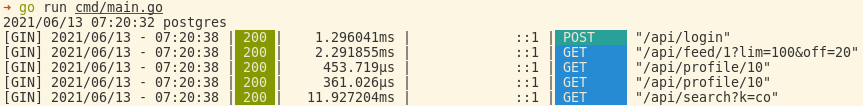
\includegraphics[width=\textwidth]{img/b1.png}
    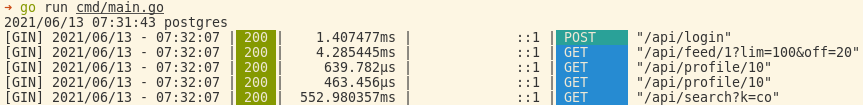
\includegraphics[width=\textwidth]{img/b2.png}
    \caption{Зависимость времени ответа на запросы от размера таблицы}
\end{figure}


\begin{verbatim}
explain analyse select * from Profile where id = 1000;

Index Scan using profile_pkey on profile
(cost=0.28..8.29 rows=1 width=335) (actual time=0.030..0.032 rows=1 loops=1)
Index Cond: (id = 1000)
Planning Time: 1.042 ms
Execution Time: 0.197 ms
\end{verbatim}

Мы видим, что время выполнения при получении профиля лишь немного увеличилось. Поскольку он выполняет поиск по pk, а столбец pk использует index. Хотя в этом случае сканирование последовательности будет даже быстрее, потому что строка находится в верхней части таблицы. Что касается функции поиска, которая представляет собой сложную функцию, использующую множество объединений, а также функцию json, время отклика увеличилось в 50 раз.


% \section{Зависимость времени ответа на запросы от размера таблицы}




% \section{Вывод}


% Из эксперимента можно сделать вывод, что программа правильно реализована.
% Хотя в точках пересечения из-за ограниченной точности числового типа «float»,
% на пересечениях иногда появляются ложные пиксели.
% Программа хорошо представляет физические свойства света,
% работает быстро (100fps) на небольших и простых сценах.
% Свойства материала отображаются не очень хорошо,
% но по сравнению с рендером в реальном времени это приемлемо.
% Алгоритм трассировки лучей позволяет нам контролировать, как свет взаимодействует с материалом объекта,
% зато количество вычислений значительно увеличивается.
